\section{Image Loading and Display}
\subsection{Loading the image}
I used the imread function to read the image. I then used the double function to convert the data type of the image to a double and finally normalized all the values to be in the range 0 - 1. The lab then required me to use the rgb2gray function to convert the RBG image to a grayscale image. This is shown below in Figure \ref{fig:RBGGrayTransform}.

\begin{figure}[h]
    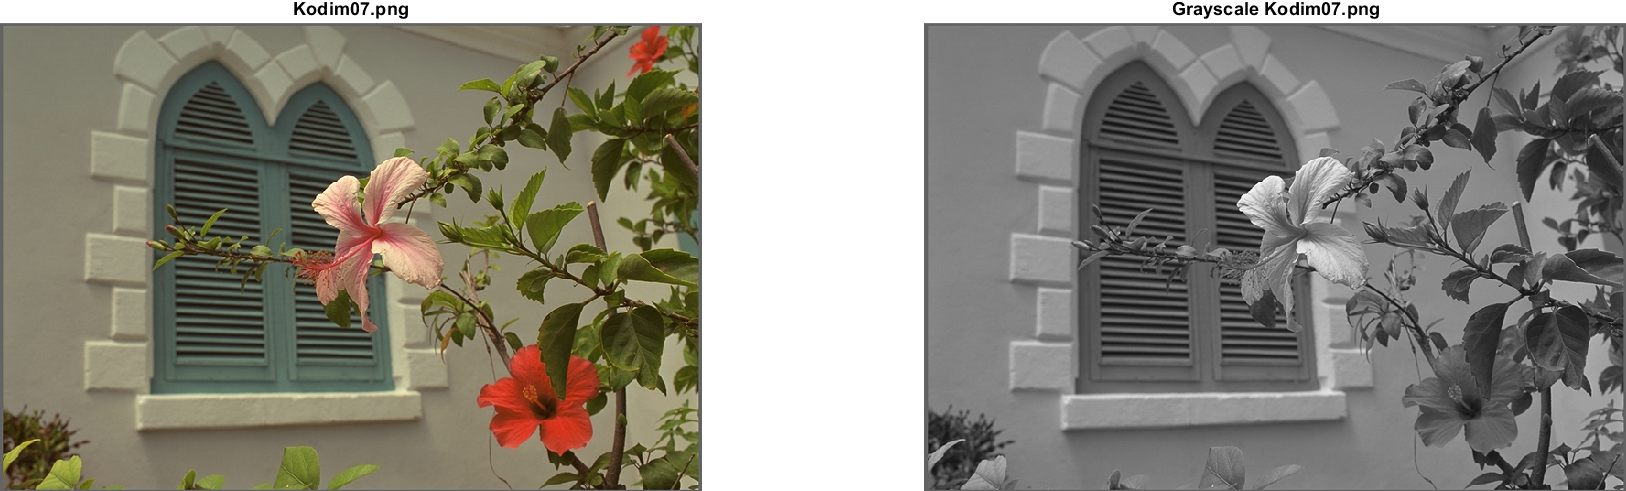
\includegraphics[width=1\textwidth]{RGBGrayscaleKodim07.png}
    \centering
    \caption{RBG and Grayscale Image}
    \label{fig:RBGGrayTransform}
\end{figure}

\subsection{Adding 128 to the pixels}
\label{sec:SubSecAdd128}
Here I had to add 128 to all the pixels in the RGB image, effectively brightening the image. However, since all the values in the image were normalized I had to add $\frac{128}{255}$ to all the pixels in the image. The output from this operation is shown below in Figure \ref{fig:128AddTransform}.

\begin{figure}[h]
    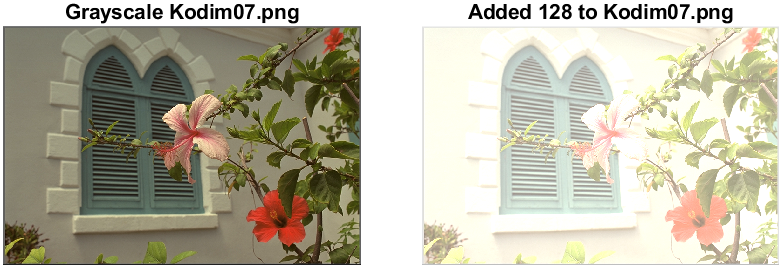
\includegraphics[width=1\textwidth]{Kodim07Add128.png}
    \centering
    \caption{Adding 128 to the RGB Image}
    \label{fig:128AddTransform}
\end{figure}

As can be seen from Figure \ref{fig:128AddTransform}, a lot of the pixels that were gray in the normal image turned white, or close to white, after the transformation. This is because colors that are gray or close to gray, have RGB values that are around (128, 128, 128). Adding 128 to these pixels means that their RGB values come close to (255, 255, 255) which corresponds to white.

\subsection{Subtracting 128 from the pixels}
In this exercise, I had to subtract 128 from all the pixels. This was performed in a similar manner to exercise \ref{sec:SubSecAdd128}. The result of this operation is shown in Figure \ref{fig:128SubTransform}. Pixels that have a value of gray or close to gray in the original image now appear black since they have their RBG values pushed to (0, 0, 0) after the transformation. This also has the effect of darkening the image when compared with the original.
\pagebreak
\begin{figure}[h]
    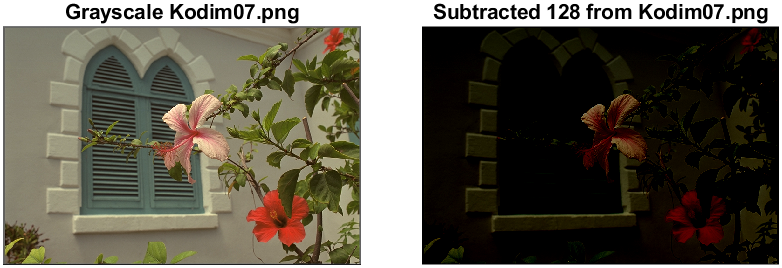
\includegraphics[width=1\textwidth]{Kodim07Sub128.png}
    \centering
    \caption{Subtracting 128 from the RGB Image}
    \label{fig:128SubTransform}
\end{figure}

